%%
%% Sem4Tra 2026 -- Seventh International Workshop on Semantics for Transport and Logistics
%% Co-located with the SEMANTiCS Conference 2026, Ghent, 15 September 2026.
%%
%% This paper uses the CEURART one-column style (ceurart.cls).
%% The class file ceurart.cls is provided by the Overleaf CEUR-WS template:
%%   https://www.overleaf.com/latex/templates/template-for-submissions-to-ceur-workshop-proceedings-ceur-ws-dot-org/wqyfdgftmcfw
%%
\documentclass[twocolumn]{ceurart}

%%
%% Additional packages used by the figures in this paper.
%%
\usepackage{tikz}
\usetikzlibrary{arrows.meta,positioning,shapes.geometric,calc,fit,backgrounds}
\usepackage{booktabs}
\usepackage{listings}
\usepackage{xcolor}
\usepackage{xurl}

%% Lightweight code listing style for SPARQL/SQL snippets.
\definecolor{codebg}{RGB}{245,245,245}
\definecolor{codekw}{RGB}{0,0,160}
\definecolor{codecm}{RGB}{100,100,100}
\lstset{
  basicstyle=\ttfamily\scriptsize,
  backgroundcolor=\color{codebg},
  keywordstyle=\color{codekw}\bfseries,
  commentstyle=\color{codecm}\itshape,
  breaklines=true,
  columns=fullflexible,
  frame=none,
  showstringspaces=false,
  keepspaces=true,
  aboveskip=4pt,
  belowskip=4pt,
}
\lstdefinelanguage{sparql}{
  morekeywords={CONSTRUCT,WHERE,SELECT,INSERT,DELETE,SERVICE,BIND,VALUES,UNION,OPTIONAL,FILTER,AS,PREFIX,a},
  morecomment=[l]{\#},
  morestring=[b]",
}

%%
%% Reusable TikZ styles.
%%
\tikzset{
  box/.style   = {rectangle, rounded corners=2pt, draw, thick, align=center,
                  font=\scriptsize, inner sep=3pt, minimum height=7mm},
  kg/.style    = {circle, draw, thick, align=center, font=\scriptsize,
                  fill=green!12, minimum size=12mm},
  db/.style    = {cylinder, shape border rotate=90, aspect=0.25, draw, thick,
                  align=center, font=\scriptsize, fill=red!10, minimum height=8mm},
  flow/.style  = {-{Stealth[length=2mm]}, thick},
  dflow/.style = {-{Stealth[length=2mm]}, thick, dashed},
}

\begin{document}

%%
%% Copyright / conference metadata.
%%
\copyrightyear{2026}
\copyrightclause{Copyright for this paper by its authors.
  Use permitted under Creative Commons License Attribution 4.0
  International (CC BY 4.0).}

\conference{Sem4Tra 2026: Seventh International Workshop on Semantics for
  Transport and Logistics, co-located with the SEMANTiCS Conference 2026,
  September 15, 2026, Ghent, Belgium}

\title{Building and Publishing a Railway Infrastructure Knowledge Graph:
  Lessons Learned from SPARQL Anything, GeoSPARQL, SHACL and RINF Publication}

%%
%% Authors. Adjust ORCID / e-mail / affiliation as needed.
%%
\author[1]{Mathias~{Vanden Auweele}}[
  orcid=0009-0004-4838-7029,
  email=mathias@matdata.eu,
]

\author[2]{Linnea Catharina Olsen}[
  email=linnea.catharina.olsen@banenor.no,
]

\author[2]{Mia Pin Berge}[
  email=mia.pin.berge@banenor.no,
]

\author[2]{Johan Korsmo}[
  email=johan.korsmo@banenor.no,
]

\address[1]{Matdata, Belgium}
\address[2]{Bane NOR, Norway}

\cortext[1]{Corresponding author.}

%%
%% Abstract.
%%
\begin{abstract}
  Railway infrastructure data is fragmented across topology models, asset
  systems, engineering systems, geographic information systems and regulatory
  datasets; the same railway is represented differently in each. A knowledge
  graph offers a semantic integration layer that unifies these silos around a
  shared model. We report on the construction and publication of a
  production railway infrastructure knowledge graph for the Norwegian
  infrastructure manager, comprising roughly 13 million triples across
  seventeen ontologies and covering more than five thousand kilometres of
  track. Unlike many geospatial domains, railway infrastructure is
  fundamentally \emph{topology-based}: assets are positioned through linear
  referencing and route-based coordinates rather than absolute geometry. We
  describe a pragmatic ingestion pipeline built on SPARQL Anything, the
  evolution from post-processing SPARQL queries towards declarative SHACL
  rules, and the generation of a European Register of Infrastructure (RINF)
  export directly from the graph. Our central finding is that, while SPARQL
  Anything, SHACL and GeoSPARQL enable much of the required functionality, our
  experience demonstrates that railway infrastructure knowledge graphs require
  stronger support for topology-based modelling, routing and linear
  referencing than is currently available in mainstream Semantic Web tooling.
  As a consequence, a significant amount of spatial and topological logic had
  to remain in SpatiaLite SQL or in custom Python scripts outside the graph -- 
  an observation we believe is relevant to the wider community.
\end{abstract}

\begin{keywords}
  Knowledge Graph \sep
  Railway Infrastructure \sep
  SPARQL Anything \sep
  GeoSPARQL \sep
  SHACL \sep
  Linear Referencing \sep
  Topology \sep
  RINF \sep
  GIS 
\end{keywords}

\maketitle

%% =====================================================================
\section{Introduction}
%% =====================================================================

\subsection{Problem}

A railway infrastructure manager is responsible for far more than running
trains on time. The infrastructure itself -- thousands of kilometres of track,
together with signals, switches, bridges, tunnels and overhead lines -- must be
built, maintained, renewed and planned decades ahead. A wide range of business
domains depend on accurate and consistent infrastructure data: asset
maintenance (track, catenary, signalling, telecoms, structures), infrastructure
projects (ERTMS rollout, track renewal, station upgrades), operations (traffic
management, capacity planning, timetabling, simulation), stakeholder
communication (train operators, regulators, the public) and corporate functions
(finance, contracts, procurement).

Historically, each of these use cases evolved its own application, its own data
model and its own copy of the infrastructure. The result is dozens of
overlapping, inconsistent representations of the \emph{same} railway --
sometimes so divergent that they appear to describe a different railway
entirely. Changes made in one system do not propagate to the others;
reconciliation is manual and error-prone. Railway infrastructure data thus
exists simultaneously in topology models, asset systems, engineering systems,
geographic information systems (GIS) and regulatory datasets, each with its own
identifiers, granularity and assumptions.

A knowledge graph offers a semantic integration layer over these silos: a
single, authoritative model of the infrastructure that can serve reference data
to all use cases from one source of truth, and that grounds transactional data
exchange in solid, shared reference data. This is the vision pursued by the
\emph{Digital Infrastructure Model} (DIM) of the Norwegian infrastructure
manager Bane NOR~\cite{dim}: consolidating data from multiple sources into one
connected model that gives all user groups access to traffic-oriented
information.

\subsection{Challenge}

Realising this vision surfaces difficulties that reach well beyond the geometric
concerns of most GIS applications. Managing railway asset and network data
involves three fundamental, generic and often neglected
complexities~\cite{dimvision}:

\begin{itemize}
  \item \textbf{Location} -- an asset must be positioned along several
        complementary dimensions: \emph{topological} (where the asset sits in
        the network graph, and thus how it affects train routing -- the most
        critical dimension), \emph{geographic} (latitude and longitude),
        \emph{linear} (a measure along a line) and \emph{address-based}
        (kilometrage).
  \item \textbf{Time} -- both the time of \emph{knowledge} (what we already know
        today about a future state of the network) and the time of
        \emph{validity} (when a change actually becomes operational) must be
        represented.
  \item \textbf{Identity} -- the identity of an entity, of its lifecycle phase (a
        distinct identifier per phase plus one canonical, phase-less identity)
        and of its aspect (for example, equipment versus function).
\end{itemize}

A production infrastructure model must ultimately address all three to become a
stable product, and a knowledge graph is well suited to doing so: it allows
independent metadata to be attached to each individual property, so that a
complex model can still expose a simple snapshot of the network through a few
rules. \emph{In this paper, however, we deliberately limit the discussion to the
first complexity, and within it to the topological and spatial dimensions of
location.} Time and identity, though equally important, are beyond our scope
here.

Even so restricted, the problem is hard, because these dimensions are only
partially supported by current Semantic Web standards. Where cadastral, utility
or generic GIS applications are primarily concerned with \emph{geometry} --
points, lines and polygons in a coordinate reference system -- railway
infrastructure relies heavily on:

\begin{itemize}
  \item \textbf{topology} -- the network as a graph of nodes and edges, with
        explicit navigability;
  \item \textbf{linear referencing} -- positioning assets along a track by a
        measure (e.g. kilometrage or an intrinsic coordinate) rather than by an
        absolute point;
  \item \textbf{route-based positioning} -- locations that only make sense along
        a path through the network.
\end{itemize}

GeoSPARQL~\cite{geosparql} is geometry-centric; it offers rich handling of
geometries, spatial predicates and coordinate reference systems, but it has no
native notion of linear referencing, kilometrage, routing or topology
traversal. As we shall show, this mismatch has practical consequences for any
railway knowledge graph built on today's tooling.

\subsection{Contribution}

This paper presents an experience report of a production railway knowledge
graph. Concretely, we contribute:

\begin{enumerate}
  \item a description of a \emph{production} railway KG construction pipeline,
        including its pragmatic workarounds (Section~\ref{sec:pipeline});
  \item lessons learned using \emph{SPARQL Anything}~\cite{sparqlanything} and
        the Facade-X~\cite{facadex} approach for ingesting heterogeneous
        railway source formats;
  \item the evolution from SPARQL post-processing towards \emph{SHACL}-based
        transformation~\cite{shacl,shaclaf} (Section~\ref{sec:shacl});
  \item the limitations we encountered with \emph{GeoSPARQL} for
        topology-centric and linear-reference-centric data
        (Section~\ref{sec:geosparql});
  \item the generation of a \emph{RINF} publication directly from the graph
        (Section~\ref{sec:rinf}).
\end{enumerate}

Our aim is not to claim a novel algorithm, but to distil what worked, what did
not, and where the Semantic Web stack falls short for a topology-driven domain.

%% =====================================================================
\section{Railway Topology as the Foundation}
\label{sec:topology}
%% =====================================================================

The single most important insight from our work is that railway infrastructure
is fundamentally topology-based. Before describing the pipeline, we explain what
this means and why it matters.

\subsection{Many Topology Models Coexist}

Unfortunately, there is no single railway topology model. Several standards
exist and are in active use at the same time, often within one organisation:

\begin{itemize}
  \item \textbf{RailTopoModel (RTM)}~\cite{rtm} -- the UIC standard, published as
        IRS~30100, that first established a topology-based foundation for
        positioning on the railway network. It models the network with net
        elements and net relations expressing navigability, at configurable
        levels of detail (micro, meso, macro). Version~1.1 is the most widely
        shared baseline; the next three models below can largely be understood 
        as forks of it.
  \item \textbf{railML~3.x}~\cite{railml} -- the XML serialisation that adopted
        RTM for positioning and then continued to develop the topology model
        under the railML umbrella (railML~3.1/3.2/3.3 tracking RTM~1.3/1.4/1.5).
        The earlier and still widely deployed \textbf{railML~2.x} generation is
        track-and-line oriented and does \emph{not} carry a full topology.
  \item \textbf{RSM (Rail System Model)}~\cite{rsm} -- UIC's own continuation of
        RTM (effectively RTM~1.2), developed after UIC and railML diverged.
  \item \textbf{ERA ontology}~\cite{eraontology,rinf} -- the European regulatory
        model behind RINF. It began as a macro-level model of operational points
        and sections of line; more recently, RTM concepts were introduced to
        support micro topology, but with renamed classes (for example
        \texttt{SpotLocation} becomes \texttt{NetPointReference}). Its topology
        is therefore \emph{inspired by} RTM but not identical to it -- a
        divergence that later causes concrete conversion problems
        (Section~\ref{sec:rinf}).
  \item \textbf{OpenTNF}~\cite{opentnf} -- an open topology network format built
        as an extension of GeoPackage~\cite{geopackage} (itself an extension of
        SQLite). Nodes represent switches and ends of track; edges represent
        track segments.
  \item \textbf{Proprietary formats} -- many operational and engineering systems
        carry their own topology and asset-positioning schemes. The authors have
        semantic-mapping experience with, among others, Hacon's TPS, TrafIT's
        railOscope and Infrabel's
        InfraNET/InfraGIS~\cite{hacontps,trafit,infrabel}, each with its own take
        on topology and positioning.
  \item \textbf{OpenStreetMap}~\cite{osm} -- a crowdsourced geometric view with
        partial and inconsistent topology.
\end{itemize}

Each model draws the network boundary differently, chooses a different
granularity, and uses different identifiers. Integrating source systems is,
therefore, fundamentally an act of mapping their base topologies onto one
unified topology. Once a shared topology exists, assets from different source
systems can coexist and relate to one another.

\subsection{Graph-Based Topology}

At its core a topology models the railway as a graph
(Figure~\ref{fig:topology}): a set of \emph{nodes} connected by \emph{edges}. 
\footnote{A crucial caveat is that this \emph{topology graph} is not the same 
thing as the \emph{knowledge graph} into which it is eventually encoded. In a 
topology graph, nodes and edges denote physical network primitives -- connection 
points and track segments. Once serialised as RDF, those primitives become 
resources, and the RDF edges (triples) instead express relationships \emph{about} 
them. In other words, nodes and edges carry a different meaning in the two graphs, 
and conflating them is a common source of confusion.}

The models also differ in how much structure they guarantee. In RTM the network
is described by \emph{net elements} connected by \emph{net relations}, and
navigability -- which movements through a node are physically possible -- is
expressed explicitly as a property of those relations, which makes RTM a good
integration target. Not every model is so disciplined: some topology models do
not represent navigability at all, and some do not restrict nodes to switches
and ends of track but instead attach signals and other assets directly into the
topology graph. The latter choice severely complicates topology maintenance,
because moving or renewing an asset then perturbs the network structure itself.

OpenTNF illustrates the practical gaps. Its nodes are switches and ends of track
and its edges are track segments, but it has no native concept of navigability;
in practice this has to be reconstructed in a proprietary manner. OpenTNF also
uses a \texttt{link\_sequence} construct -- a kind of ``super-edge'' that spans
several smaller edges -- so a necessary first ingestion step is to decompose each
link sequence back into the most basic edges before the topology can be mapped
onto the unified model.

Once navigability is present, this graph structure yields three properties that
plain geometry cannot:

\begin{itemize}
  \item \textbf{Unambiguous positioning} -- every asset has a precise, unique
        location on the network.
  \item \textbf{Clear navigability} -- the graph can be traversed to find
        routes, adjacencies and reachability.
  \item \textbf{Things, not strings} -- positioning does not rely on
        human-readable names or kilometre posts, which are ambiguous and change
        over time; it relies on the structure itself.
\end{itemize}

\begin{figure}[t]
  \centering
  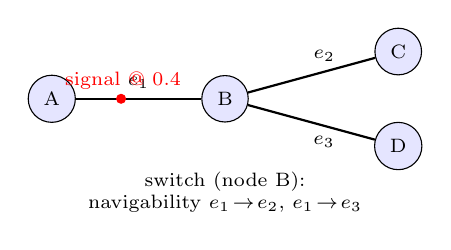
\begin{tikzpicture}[every node/.style={font=\scriptsize}]
    % nodes
    \node[circle,draw,fill=blue!10,minimum size=5mm] (a) at (0,0) {A};
    \node[circle,draw,fill=blue!10,minimum size=5mm] (b) at (2.2,0) {B};
    \node[circle,draw,fill=blue!10,minimum size=5mm] (c) at (4.4,0.6) {C};
    \node[circle,draw,fill=blue!10,minimum size=5mm] (d) at (4.4,-0.6) {D};
    % edges
    \draw[thick] (a) -- node[above,pos=0.5]{$e_1$} (b);
    \draw[thick] (b) -- node[above,pos=0.6]{$e_2$} (c);
    \draw[thick] (b) -- node[below,pos=0.6]{$e_3$} (d);
    % asset on edge e1 at intrinsic coord 0.4
    \filldraw[red] ($(a)!0.4!(b)$) circle (1.6pt);
    \node[red,above] at ($(a)!0.4!(b)$) {\,signal @ 0.4};
    % switch marker at B
    \node[below=5mm of b,align=center] {switch (node B):\\navigability
      $e_1\!\to\!e_2$, $e_1\!\to\!e_3$};
  \end{tikzpicture}
  \caption{A railway topology as a graph. Node~B is a switch connecting edges
    $e_1$, $e_2$ and $e_3$. The signal is positioned by an intrinsic
    coordinate ($0.4$) along edge $e_1$, not by an absolute point.}
  \label{fig:topology}
\end{figure}

\subsection{Asset Positioning}

Assets in source systems are still typically recorded by their absolute
geometric position (or worse.. with a kilometric position...), but what matters 
for railway operations is their \emph{topological} position, because that is what 
determines how an asset affects train traffic. The distinction is not academic: 
a signal may physically stand closer to a neighbouring track than to the track it 
actually governs, so a purely geometric ``nearest track'' assignment would attach 
it to the wrong edge. Only an explicit topological position captures the intended 
meaning.

When positioning assets against a topology, three complementary methods appear
throughout the data:

\begin{itemize}
  \item \textbf{Intrinsic coordinates} -- the asset is bound to one or more net
        elements through an associated-net-element reference, with an intrinsic
        coordinate (a value between $0$ and $1$) giving its relative position
        along an edge. A signal ``at $0.4$ on edge $e_1$'' is unambiguous
        regardless of the edge's absolute geometry. This is the most important
        method, being the only one intrinsically tied to the topology.
  \item \textbf{Geometric coordinates} -- ordinary spatial coordinates, but used
        as a reference to the topological position rather than to the true
        physical location of the asset. Keeping a geometry that follows the track
        makes visual representation easy while the position remains
        topologically meaningful.
  \item \textbf{Linear coordinates} -- a measure along a linear positioning
        system. Depending on that system, the measure may be relative to an
        anchor (such as a kilometric post) or relative to the origin of the
        positioning system; the latter makes distance calculations between
        positions straightforward along that specific axis.
\end{itemize}

Kilometrage -- the traditional railway ``km + offset'' notation -- deserves a
specific warning. Although it superficially resembles a linear referencing
system~\cite{lrs}, in practice it is so riddled with misuse and hidden issues (it
resets at boundaries, contains gaps and overlaps, and changes when a line is
re-surveyed) that it is safest to treat it as a mere \emph{addressing} system
rather than a reliable measure to compute with.

%% =====================================================================
\section{Knowledge Graph Construction Pipeline}
\label{sec:pipeline}
%% =====================================================================

We now describe how the graph is built. To keep the focus on the semantic
lessons, we deliberately omit the operational plumbing (orchestration,
scheduling, clustering) and present a simplified view. The pipeline is mature
and runs in production: it currently produces roughly 13 million triples
across seventeen ontologies, covering more than five thousand kilometres of
track~\cite{dim}.

\subsection{The Vision Versus the Reality}

We set out to build a simple three-step pipeline: multiple heterogeneous source
systems feed a single knowledge graph, from which railML files are generated for
downstream use cases. The railML files act as a bridge, so that existing tools
keep working without modification while use cases gradually move towards
consuming RDF directly. Reality required considerably more machinery, summarised
in Figure~\ref{fig:pipeline}.

\subsection{Choosing a Base Railway Ontology}

No single railway ontology covers all of our requirements, so the choice of a
base vocabulary was a deliberate trade-off. We selected the railML
ontology~\cite{railmlontology} as the backbone for railway-specific concepts. It
is derived from the railML schema, a mature and proven exchange format that
already covers a broad catalogue of documented railway use
cases~\cite{railmlusecases}, and it inherits the solid RTM foundation for
topology (Section~\ref{sec:topology}). Although the \emph{ontology} is still
under active development, the underlying \emph{schema} is very stable, which
gives us confidence in the modelling. By contrast, the ERA
ontology~\cite{eraontology}, while mandated for regulatory publication, does not
yet have a comparable track record of proven use cases; we therefore treat it as
an export target (Section~\ref{sec:rinf}) rather than as our internal backbone.

For the many generic, non-railway-specific aspects we reuse established W3C and
community ontologies rather than reinventing them: OWL-Time for temporal
entities, QUDT for quantities and units, SKOS for code lists and concept schemes,
GeoSPARQL for geometry, schema.org and Dublin Core Terms for descriptive
metadata, and PROV for provenance. This keeps the railway-specific vocabulary
small and lets standard tooling operate on the generic parts of the graph.

\subsection{Data Ingestion with SPARQL Anything}

Our team was new to knowledge graph construction and evaluated several mapping
approaches (R2RML~\cite{r2rml}, RML~\cite{rml}, custom code). The decisive factor
was that we already had to learn SPARQL for querying the graph -- so why learn
yet another mapping language? SPARQL Anything~\cite{sparqlanything} lets us write
\texttt{CONSTRUCT} queries that map source data into RDF through the Facade-X
lens~\cite{facadex}, using a single language for both mapping and querying. Our
primary source formats are XML, CSV and the OpenTNF/GeoPackage database.

The authoritative source turned out not to be raw railML~2.x XML (which was
incomplete and carried no topology) but OpenTNF, whose spatial foundation is a
topology. Because SPARQL Anything operates on files rather than databases, we
built a \emph{Source Ingestor} that exports the relevant SQL tables to CSV. The
ingestor later took on additional responsibilities (Sections~\ref{sec:shacl}
and~\ref{sec:geosparql}). Each exported CSV is asset-based (one file per asset
type -- switches, signals, balises, speed sections, and so on), and each is
mapped by one \texttt{CONSTRUCT} query. The mapping layer covers roughly forty
asset types. Listing~\ref{lst:construct} shows the recurring pattern.

\begin{lstlisting}[language=sparql,caption={Asset mapping with SPARQL Anything: a
  \texttt{SERVICE} clause reads a CSV through Facade-X; the \texttt{CONSTRUCT}
  builds railML/RTM triples and positions the asset by intrinsic
  coordinate.},label={lst:construct}]
CONSTRUCT {
  ?balise a railml3:Balise, rtm:NetEntity ;
    rdfs:label ?label ;
    rtm:hasSpotLocation ?loc .
  ?loc a rtm:SpotLocation ;
    rtm:onNetElement ?netelement ;
    rtm:hasIntrinsicCoordinate ?coord .
}
WHERE {
  SERVICE <x-sparql-anything:location=
      balises.csv,csv.headers=true> {
    ?s xyz:atb_banedata_id ?id ;
       xyz:name ?label ;
       xyz:measure_on_link ?coord .
  }
  BIND(IRI(CONCAT(STR(bnd:),
      "_balise_", STR(?id))) AS ?balise)
}
\end{lstlisting}

\subsection{Loading, Post-Processing and Export}

The generated Turtle is loaded into an Apache Jena TDB2 dataset and served
through Fuseki~\cite{jena} as a SPARQL endpoint. Because a single pass of
\texttt{CONSTRUCT} mapping is not enough (see Section~\ref{sec:shacl}), a series
of post-processing queries runs against the freshly loaded graph, followed by
fifteen sequential \emph{splitting} queries that extract subnetworks for railML
export. Crucially, all of this post-processing takes place on a \emph{staging}
TDB2 dataset; only once post-processing has completed successfully do we
\emph{hot-swap} the finished dataset behind the stable endpoint name, so that the
graph can be updated without ever exposing consumers to a partially processed
state.

\begin{figure*}[t]
  \centering
  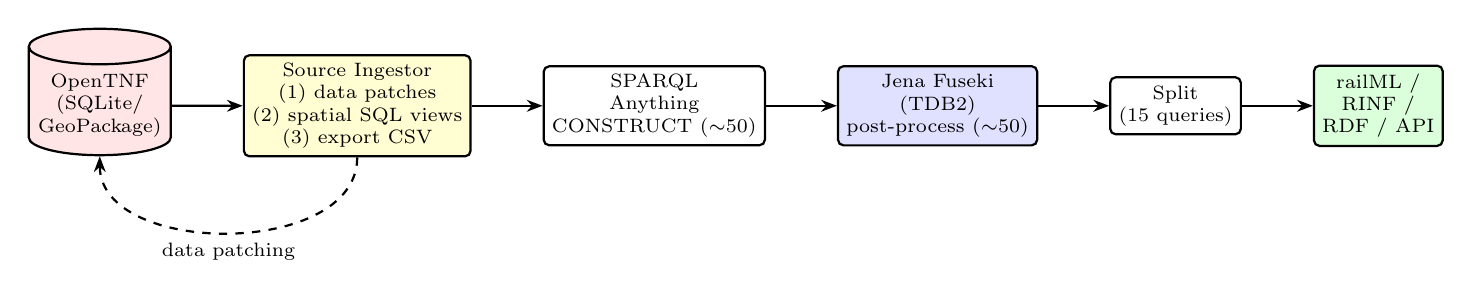
\begin{tikzpicture}[node distance=6mm and 9mm]
    \node[db] (tnf) {OpenTNF\\(SQLite/\\GeoPackage)};
    \node[box, right=of tnf, fill=yellow!18] (si)
      {Source Ingestor\\\scriptsize (1) data patches\\(2) spatial SQL views\\(3) export CSV};
    \node[box, right=of si] (sa) {SPARQL\\Anything\\\scriptsize CONSTRUCT ($\sim$50)};
    \node[box, right=of sa, fill=blue!12] (fus)
      {Jena Fuseki\\(TDB2)\\\scriptsize post-process ($\sim$50)};
    \node[box, right=of fus] (split) {Split\\\scriptsize (15 queries)};
    \node[box, right=of split, fill=green!14] (out) {railML /\\RINF /\\RDF / API};

    \draw[flow] (tnf) -- (si);
    \draw[flow] (si) -- (sa);
    \draw[flow] (sa) -- (fus);
    \draw[flow] (fus) -- (split);
    \draw[flow] (split) -- (out);
    \draw[dflow] (si.south) to[out=-90,in=-90] node[below,font=\scriptsize]{data patching} (tnf.south);
  \end{tikzpicture}
  \caption{Simplified production pipeline. The Source Ingestor performs data
    patches and spatial SQL before export; SPARQL Anything maps CSV to RDF;
    Jena Fuseki hosts the graph and runs post-processing; splitting queries
    extract subnetworks for railML and RINF export. Orchestration is omitted
    for clarity.}
  \label{fig:pipeline}
\end{figure*}

%% =====================================================================
\section{Semantic Transformation with SHACL}
\label{sec:shacl}
%% =====================================================================

A recurring theme in our work is \emph{where} semantic transformation should
happen. This section traces that evolution, which we consider more instructive
than the mapping queries themselves.

\subsection{Initial Approach: SPARQL CONSTRUCT}

Initially, all mapping was performed with \texttt{CONSTRUCT} queries at ingestion
time (Listing~\ref{lst:construct}). This works well for single-file,
asset-by-asset mappings and gives a low entry barrier. It breaks down, however,
as soon as relationships span multiple source files. Inferring where a track
begins and ends, for example, requires resolving how tracks connect through
switches and buffer stops across several asset files -- awkward to express with
nested \texttt{SERVICE} clauses in SPARQL Anything, which reads one file at a
time.

\subsection{Evolution: Post-Processing Queries}

We therefore moved cross-cutting logic into post-processing
\texttt{INSERT}/\texttt{DELETE} queries that run against the fully loaded graph.
This solved two problems: (i) cross-file relationships, now expressible over the
assembled graph; and (ii) generalised actions applied uniformly to many entity
types -- for example completing or normalising values that individual mapping
queries left implicit. Listing~\ref{lst:postproc} shows a representative case:
deriving the missing \texttt{time:inXSDDate} of a time instant from its
\texttt{time:inXSDDateTimeStamp}, applied uniformly to every instant in the
graph.

\begin{lstlisting}[language=sparql,caption={Representative post-processing: a
  generalised \texttt{INSERT} that completes the missing date on any
  \texttt{time:Instant} from its timestamp, applied uniformly across the whole
  graph.},label={lst:postproc}]
INSERT {
  ?instant time:inXSDDate ?date .
}
WHERE {
  ?instant a time:Instant ;
    time:inXSDDateTimeStamp ?dateTimeStamp .
  FILTER NOT EXISTS {
    ?instant time:inXSDDate ?d . }
  BIND(STRDT(SUBSTR(STR(?dateTimeStamp), 1, 10),
    xsd:date) AS ?date)
}
\end{lstlisting}

The cost of this approach becomes apparent at scale. We accumulated roughly
fifty post-processing queries that must run in a specific order, because some
steps depend on the output of earlier ones. The dependencies are encoded only by
a numeric filename prefix and comments; there is no explicit dependency graph, no
validation that a step's preconditions hold, and no lineage recording which
source triples produced which derived triples. In effect, the post-processing
layer is an imperative program written in SPARQL.

Earlier iterations of the pipeline also performed multi-ontology mapping in this
layer, adding ERA types alongside railML ones in the same post-processing step.
We have since moved away from that: mixing regulatory ERA mapping into general
post-processing meant many different semantic actions happened at once, which
increased complexity. Conversion to the ERA ontology is now done
\emph{exclusively} in the RINF export through SHACL-AF rules
(Section~\ref{sec:rinf}), keeping the post-processing layer focused on
graph-internal completion.

\subsection{Future Direction: SHACL Rules}

The natural next step is to replace ad-hoc post-processing with declarative SHACL
rules~\cite{shacl,shaclaf}: first ingest a raw, faithful graph that mirrors the
source structure, triplified according to Facade-X~\cite{facadex}\footnote{We will
deviate slightly from the default Facade-X metamodel towards a 
``one-eyed graph''~\cite{oneeyedgraph} which will improve SHACL rule readability.},
then apply SHACL rules to perform the semantic mapping to the target ontologies.
In our pipeline this is already in use for the regulatory RINF export, where
target properties are derived through SHACL-AF rules and validated against ERA's
official shapes before each export.

Listing~\ref{lst:shaclrule} shows a representative rule from that export. It
targets the railML-centred graph and mints the corresponding ERA entity: every
operational point carrying a primary-location-code (PLC) designator becomes an
\allowbreak\mbox{\texttt{era:PrimaryLocation}} in the RINF-oriented view.

\begin{lstlisting}[language=sparql,caption={A SHACL-AF rule mapping the
  railML-centred graph towards the RINF/ERA view: each operational point with a
  PLC designator yields an \allowbreak\mbox{\texttt{era:PrimaryLocation}}. The rule is attached to
  a node shape whose target selects the currently valid operational
  points.},label={lst:shaclrule}]
bnd:_rule_mint_primary_location
  a sh:SPARQLRule ;
  sh:prefixes bnd:_prefixes ;
  sh:construct """
    CONSTRUCT {
      ?pl a era:PrimaryLocation ;
        era:primaryLocationCode ?plc ;
        era:primaryLocationName ?label .
    }
    WHERE {
      $this rdfs:label ?label ;
        railml3:hasDesignator ?d .
      ?d railml3:hasEntry ?plc ;
         railml3:hasRegister "PLC" .
      BIND(IRI(CONCAT(STR(bnd:),
        "_primaryLocation_", ?plc)) AS ?pl)
    }
  """ .
\end{lstlisting}

The advantages align well with current Semantic Web discussions:

\begin{itemize}
  \item \textbf{Separation of concerns} -- ingestion is decoupled from semantic
        mapping, so each can evolve independently.
  \item \textbf{Maintainability} -- rules are declarative shapes rather than an
        ordered pile of imperative queries. Their execution order is not
        hand-coded but determined by the rules engine, which builds a dependency
        graph over the rules and typically applies them repeatedly until a
        fixpoint is reached and no new triples are inferred.
  \item \textbf{Lineage} -- the rules are themselves triples in the graph and can
        therefore be annotated, which makes it natural to record which rule and
        which source triples justify each derived triple.
  \item \textbf{Validation and transformation together} -- the same shape
        language expresses both what is valid and how to derive missing facts,
        and can drive API generation and dereferencing.
\end{itemize}

The main obstacle is tooling maturity: we return to this in
Section~\ref{sec:discussion}.

%% =====================================================================
\section{RINF Publication}
\label{sec:rinf}
%% =====================================================================

The European Register of Infrastructure (RINF) is a common register maintained
by the European Union Agency for Railways, into which every infrastructure
manager must report a defined set of infrastructure
properties~\cite{rinf,rinf_reg}. RINF exists for \emph{interoperability}: it
enables cross-border reporting, route compatibility checks and Europe-wide
digital services.

Our approach is to generate the RINF export directly from the knowledge graph
rather than maintaining it as a separate dataset. Rather than pre-computing
ERA-ontology views, \emph{all} mapping from the railML-centred graph to the ERA
vocabulary~\cite{eraontology} happens during SHACL-AF rule execution at export
time: the mandatory RINF element types -- tracks, signals, tunnels, bridges and
train detection systems -- and their required properties are derived by the rules
and validated against ERA's official shapes before submission~\cite{dim}.
Coverage is still growing: at the time of writing roughly half of the mandatory
RINF properties are mapped, with the remainder in active development.

The benefits are partly organisational. Generating RINF from the graph avoids
duplicate maintenance: there is a single source of truth, and regulatory
reporting becomes a \emph{view} of the infrastructure model rather than a
parallel dataset that can drift out of sync. Beyond that, performing the
transformation in SHACL brings a documentation benefit: because the rules are
declarative and are themselves part of the graph, they document the data lineage
of the export far better than an opaque procedural exporter would
(Section~\ref{sec:shacl}). The value is not limited to the export product,
either: by adding the inferred ERA triples back into the DIM graph, data
consumers of the underlying graph gain new perspectives and additional data, so
the regulatory mapping doubles as an enrichment of the model for all users.

The mapping also exposed a genuine difficulty: RTM and ERA take fundamentally
different approaches to asset topology locations. A lean RTM
\texttt{LinearLocation} that simply references its associated net elements must
be expanded into ERA's \texttt{NetLinearReference}, an ordered RDF-list structure
whose generating SHACL rules run to many hundreds of lines for what is
conceptually the same information. This conversion cost is a direct consequence
of the two models having diverged (Section~\ref{sec:topology}); a single, shared
approach to topology and positioning across the industry would remove an entire
class of such complicated conversions.

Notably, this approach enabled the first submission of RINF data at the micro
(topology) level of detail~\cite{dim}, made possible precisely because the
underlying graph is topology-based. This section demonstrates impact rather than
novelty: it shows that a topology-centred KG can satisfy a real regulatory
obligation as a by-product of good modelling.

%% =====================================================================
\section{GeoSPARQL and Railway Infrastructure: Lessons Learned}
\label{sec:geosparql}
%% =====================================================================

We consider this the most important section for the community. GeoSPARQL is the
natural candidate for spatial reasoning in an RDF graph, and we adopted it
expecting to perform our spatial operations inside SPARQL. In practice, a large
share of the spatial and topological logic had to remain in SQL~\cite{spatialite}. 
This section explains why.

\subsection{Railway Spatial Requirements}

Our pipeline needs the following spatial and topological operations:

\begin{itemize}
  \item \textbf{Linear referencing} -- converting between intrinsic coordinates,
        measures and absolute points along an edge (projecting an asset onto a
        track, or locating a measured position).
  \item \textbf{Kilometrage} -- handling the discontinuous ``km + offset''
        reference system.
  \item \textbf{Routing} -- finding paths through the topology respecting
        navigability at switches.
  \item \textbf{Topology traversal} -- following net relations to compute
        adjacency and reachability.
  \item \textbf{Subnet extraction} -- selecting the subgraph for a line or
        operational area together with all assets positioned on it.
  \item \textbf{Coordinate reference system (CRS) transformation} -- converting
        geometries between the coordinate reference systems used by the various
        source systems and by the published outputs.
\end{itemize}

\subsection{What GeoSPARQL Supports Well}

GeoSPARQL~\cite{geosparql} is strong at what it was designed for. It offers a
well-defined geometry model (WKT/GML literals), a comprehensive set of spatial
predicates (topological relations such as \texttt{sfIntersects},
\texttt{sfWithin}, and distance/buffer functions) and proper coordinate
reference system handling. For classic ``does this asset fall within this
region'' or ``how far apart are these two points'' questions, it is entirely
adequate -- provided the spatial operations are implemented correctly by the
SPARQL engine, which is not always a given -- and we use it where geometry is
genuinely the right abstraction.

\subsection{What Required Workarounds}

The requirements above, however, are not geometry questions -- they are linear
referencing, routing and topology questions, and GeoSPARQL has no native
vocabulary or functions for them. We therefore fell back to SpatiaLite SQL,
which does provide the necessary primitives (\mbox{\texttt{ST\_ClosestPoint}},
\allowbreak\mbox{\texttt{ST\_Line\_Locate\_Point}},
\allowbreak\mbox{\texttt{ST\_Azimuth}},
\allowbreak\mbox{\texttt{Line\_Substring}},
\allowbreak\mbox{\texttt{ST\_Reverse}},
\allowbreak\mbox{\texttt{ST\_AddMeasure}},
\allowbreak\mbox{\texttt{ST\_TrajectoryInterpolatePoint}}). Concrete examples include:

\begin{itemize}
  \item \textbf{Switch branch determination} -- deciding whether a branch turns
        left or right by comparing the azimuths of the track segments meeting at
        a switch node (Listing~\ref{lst:switch}). This requires extracting a
        short substring of each edge near the node and computing its bearing.
  \item \textbf{Line substring calculations} -- cutting an edge between two
        measures to obtain the geometry of a linear location.
  \item \textbf{Route extraction} -- assembling an ordered path through several
        edges.
  \item \textbf{Asset projection} -- projecting an asset's absolute point onto
        the nearest track to obtain its measure.
  \item \textbf{Trajectory calculations} -- interpolating a position along a
        measured trajectory.
  \item \textbf{Ordering of segments} -- placing linearly connected segments in
        the correct sequence, so that a chain of edges reads as a continuous
        route rather than an unordered set.
\end{itemize}

Most striking of all, GeoSPARQL lacks even the most elementary accessors: there
is no standard function to extract the $X$, $Y$ or $Z$ ordinate of a geometry (no
\texttt{ST\_X}, \texttt{ST\_Y} or \texttt{ST\_Z} equivalent). Obtaining a raw
coordinate value -- a trivial one-liner in any spatial SQL dialect -- therefore
already forces a detour outside the graph or a very ugly regex.

\begin{lstlisting}[language=SQL,caption={Switch branch determination in
  SpatiaLite: the direction of a branch is derived from the azimuth of a short
  substring of each track segment near the switch node -- an operation with no
  GeoSPARQL equivalent.},label={lst:switch}]
SELECT node_oid,
  ST_Azimuth(
    ST_StartPoint(seg),
    ST_EndPoint(seg)) AS bearing
FROM (
  SELECT Line_Substring(
    centreline_geom,
    0,
    MIN(20 / ST_Length(centreline_geom), 1)
  ) AS seg, node_oid
  FROM track_segments
);
\end{lstlisting}

\subsection{Consequence}

The consequence is that a significant amount of logic that conceptually belongs
to the graph had to remain in SpatiaLite SQL, executed \emph{before} data reaches
SPARQL Anything. This is not merely inconvenient: it splits the model across two
paradigms, forces spatial pre-computation ahead of semantic mapping, and means
that the graph consumer cannot ask topological or linear-referencing questions
directly. We regard this as an important observation for the community: the gap
is not in the expressiveness of RDF or SPARQL as such, but in the absence of
standardised, well-implemented linear-referencing and topology functions in the
geospatial layer of the stack.

Topology-based traversal in plain SPARQL is possible but painful. The subnet
extraction queries initially relied on many nested \texttt{OPTIONAL} clauses with
predicates bound to variables -- effectively path-finding through the graph. We
ultimately had to decompose them into fifteen sequential queries to make them
tractable, an outcome that again reflects the absence of first-class topology
support.

%% =====================================================================
\section{Discussion}
\label{sec:discussion}
%% =====================================================================

We synthesise the lessons per technology.

\subsection{SPARQL Anything}

\paragraph{Strengths.} A low entry barrier for a team new to RDF; rapid
development; and, crucially, the direct use of SPARQL for both mapping and
querying, avoiding a second mapping language. For file-based, asset-by-asset
mapping it is highly effective, and Facade-X~\cite{facadex} provides a uniform
lens over heterogeneous formats.

\paragraph{Weaknesses.} It operates on files, not databases, which forced us to
build the Source Ingestor to export CSV. Cross-file relationships are hard to
express with nested \texttt{SERVICE} clauses -- though this weakness is largely
overcome by using SPARQL Anything (and its Facade-X metamodel) purely to
triplify the sources into a faithful one-eyed graph first, and then expressing
the cross-file semantic transformation as SHACL-AF rules over the assembled
graph rather than inside the mapping queries. Left unchecked, the large mapping
surface ($\sim$40 asset types plus $\sim$50 post-processing queries) otherwise
becomes an imperative program that is difficult to maintain, order and reason
about.

\subsection{SHACL}

\paragraph{Strengths.} Declarative mappings via rules; validation and
transformation in one language; better maintainability than ordered SPARQL
scripts; natural lineage and impact analysis; and the potential to drive API
generation and URI dereferencing from the same shapes. In our RINF export, SHACL
already both derives and validates properties~\cite{dim}.

\paragraph{Weaknesses.} Tooling maturity -- though this has improved markedly. At
least two engines can execute SHACL rules at production scale: TopBraid
SHACL~\cite{topbraidshacl} and maplib~\cite{maplib}. We adopted the latter: on
our workload it is exponentially faster than TopBraid and employs a strong
dependency-graph algorithm to order rule execution automatically. What is still
missing is first-class data-lineage, geosparql with linear referencing and
impact-analysis support, together with richer validation tooling that lets us inspect 
and manage results -- summaries by type, trends over time, and links to work items -- 
rather than merely producing a conformance report.

\subsection{GeoSPARQL}

\paragraph{Main finding.} Current GeoSPARQL implementations are
\emph{geometry-centric}, whereas railway infrastructure modelling is largely
\emph{topology-centric} and \emph{linear-reference-centric}. GeoSPARQL handles
geometries, spatial predicates and coordinate reference systems relatively well, 
but it offers no native support for linear referencing, kilometrage, routing or
topology traversal. As a result, spatial logic that ought to live in the graph
was pushed down into SpatiaLite SQL. We believe this is the crux of the mismatch
between the Semantic Web stack and the railway domain, and the strongest
conclusion we can offer.

%% =====================================================================
\section{Future Work}
\label{sec:future}
%% =====================================================================

Our lessons point to a clearer target architecture and a concrete wish list for
the community.

\paragraph{Facade-X + SHACL-AF rules.} We intend to fully adopt the two-stage
approach: SPARQL Anything ingests a raw, faithful ``one-eyed'' graph, and SHACL
rules perform the semantic mapping to railML and ERA views, with lineage
recorded throughout. Figure~\ref{fig:future} contrasts this with today's
pipeline.

\begin{figure}[t]
  \centering
  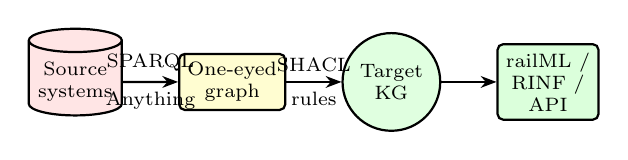
\begin{tikzpicture}[node distance=5mm and 7mm]
    \node[db] (src) {Source\\systems};
    \node[box, right=of src, fill=yellow!18] (oeg) {One-eyed\\graph};
    \node[kg, right=of oeg] (tkg) {Target\\KG};
    \node[box, right=of tkg, fill=green!14] (out) {railML /\\RINF /\\API};
    \draw[flow] (src) -- node[above,font=\scriptsize]{SPARQL} node[below,font=\scriptsize]{Anything} (oeg);
    \draw[flow] (oeg) -- node[above,font=\scriptsize]{SHACL} node[below,font=\scriptsize]{rules} (tkg);
    \draw[flow] (tkg) -- (out);
  \end{tikzpicture}
  \caption{Target architecture: faithful ingestion into a one-eyed graph,
    followed by declarative SHACL-based semantic mapping with lineage. Spatial
    pre-processing and ad-hoc post-processing queries are eliminated once the
    tooling gaps are closed.}
  \label{fig:future}
\end{figure}

\paragraph{SHACL-first transformations.} Replacing the $\sim$50 ordered
post-processing queries with declarative SHACL rules, supported by a performant
rules engine and lineage/impact-analysis tooling.

\paragraph{Linear referencing support in GeoSPARQL.} The single change that would
most simplify our work is native linear referencing~\cite{lrs} in GeoSPARQL,
properly implemented in a triple store such as Jena~\cite{jena} or an RDF library
such as maplib~\cite{maplib}. This would let us move asset projection,
line-substring and measure conversions from SQL pre-processing into SPARQL.

\paragraph{Topology-aware query functions.} Complementary to linear referencing,
standardised functions for routing, topology traversal and subnet extraction
would make the topology a first-class citizen of the query layer, removing the
need to decompose traversals into long sequential query chains.

If these gaps were closed, the split-paradigm pipeline of
Section~\ref{sec:pipeline} could collapse into the clean architecture of
Figure~\ref{fig:future}. The DIM portal~\cite{dim} serves as a lighthouse for
this direction: it already demonstrates infrastructure data consumed directly
from the triple store, and the first micro-level RINF submission shows that a
topology-based knowledge graph can meet real regulatory and interoperability
needs today.

%% =====================================================================
\begin{acknowledgments}
  We thank the Bane NOR Digital Infrastructure Model (DIM) team and the wider
  railway and Semantic Web communities for the discussions that shaped this
  experience report.
\end{acknowledgments}

%%
%% Declaration on Generative AI (required by CEUR-WS).
%% Adjust the statement to reflect actual usage.
%%
\section*{Declaration on Generative AI}
During the preparation of this work, the author(s) used generative AI tools for
grammar and spelling checking and for improving the readability of the text.
After using these tools, the author(s) reviewed and edited the content as needed
and take full responsibility for the publication's content.

%%
%% Bibliography.
%%
\bibliography{paper}

\end{document}
